%!TEX root = ../documentation.tex
\section{Configuration File}
\label{sec:config_file}

\begin{verbatim}
#!/bin/bash

# setting variables globally
set -a

#######################################################################
#######################################################################
#
# The following lines have to be adjusted according to the
# user's configuration.
#
#######################################################################
#######################################################################

##########################################
# Username
##########################################
conf_USER="mitseva"

##########################################
# An interface which tcpdump listens on
##########################################
conf_ETHDEVICE="eth0"

##########################################
# Home directory
##########################################
dir_HOME=$HOME

##########################################
# Main directory containing all tools
##########################################
dir_MAIN="${dir_HOME}/Documents/wfp_toolbox/WFP_Implementation/fingerprinting/"



#######################################################################
#######################################################################
# URL list generation
#######################################################################
#######################################################################

##########################################
# Firefox Profile
##########################################
dir_FF_PROFILE="/home/fop/.mozilla/firefox/ddmr1z3e.default"

##########################################
# Number (!) of Subpages to be Generated
##########################################
conf_SUBPAGES="5"

##########################################
# Timeout (in Seconds) for each Page Load
##########################################
conf_PAGELOAD_TIMEOUT="20"

##########################################
# Input Linklist for Subpage Generation
##########################################
file_URLList="./URL_List.txt"



#######################################################################
#######################################################################
# Fetch Processing (including Outlier Removal) & Feature generation
#######################################################################
#######################################################################

##########################################
# Patterns to be checked in traces
##########################################
conf_PATTERNS="Patterns.txt"

##########################################
# Clean transmission errors from traces representing background
##########################################
# available options: YES | NO
conf_DEL_TRANSMISSION_ERR="YES"
#conf_DEL_TRANSMISSION_ERR="NO"

##########################################
# Reference Format for synchronized Outlier Removal
##########################################

# available options: tcp | tls | tls-legacy | tls-nosendme | 
# 						cell | cell-nosendme | 
#						cell-legacy | cell-nosendme-legacy
#conf_OUTLIER_REFERENCE="tcp"
conf_OUTLIER_REFERENCE="tcp"
#conf_OUTLIER_REFERENCE="tls"
#conf_OUTLIER_REFERENCE="tls-legacy"
#conf_OUTLIER_REFERENCE="tls-nosendme"
#conf_OUTLIER_REFERENCE="cell"
#conf_OUTLIER_REFERENCE="cell-nosendme"
#conf_OUTLIER_REFERENCE="cell-legacy"
#conf_OUTLIER_REFERENCE="cell-nosendme-legacy"

##########################################
# "Strictness" of Outlier Removal
##########################################
# available options: Simple | Strict | Wang
conf_OUTLIER_REMOVAL="Simple"
#conf_OUTLIER_REMOVAL="Strict"
#conf_OUTLIER_REMOVAL="Wang"

##########################################
# Ignore Outlier Removal if necessary
##########################################
# available options: YES | NO
#conf_IGNORE_OUTLIER="YES"
conf_IGNORE_OUTLIER="NO"

##########################################
# Evaluated Scenario (Class Labeling differs)
##########################################
# available options: CW | OW_FG | OW_BG
conf_SETTING="CW"
#conf_SETTING="OW_FG"
#conf_SETTING="OW_BG"

##########################################
# Number (!) of Instances per Webpage
##########################################
conf_INSTANCES="40"

##########################################
# Take Random Instances if Possible
##########################################
# available options: YES | NO
conf_RANDOM_INSTANCES="YES"
#conf_RANDOM_INSTANCES="NO"

##########################################
# Used Classifier Version to Generate Features
##########################################
# available options: CUMULATIVE | SEPARATE
conf_CLASSIFIER="CUMULATIVE"
#conf_CLASSIFIER="SEPARATE"

##########################################
# Number (!) of Features per Instance (has to be even)
##########################################
conf_FEATURES="100"

##########################################
# Features are Outputted in a Single File or in Directories
##########################################
# available options: _ [Directories] | *Name* [Single File]
conf_DATASET="_"



#######################################################################
#######################################################################
# Choose functionality
#######################################################################
#######################################################################
# available options: ALL | FETCH | CALCULATE | FETCH_AND_CALCULATE | 
#					 CHECK_HS_STATE | CALCULATE_FEATURES
#conf_FUNCTION="ALL"
#conf_FUNCTION="FETCH"
#conf_FUNCTION="CALCULATE"
conf_FUNCTION="FETCH_AND_CALCULATE"
#conf_FUNCTION="CALCULATE_FEATURES"
#conf_FUNCTION="CHECK_HS_STATE"



#######################################################################
#######################################################################
# Choose format for data extraction
#######################################################################
#######################################################################
# available options: tcp tls tls-legacy tls-nosendme tls-nosendme-legacy 
#					 cell cell-legacy cell-nosendme cell-nosendme-legacy
#					 Wang-cell
conf_FORMATS="tcp"



##########################################
# Do backup of intermediate results
##########################################
# available options: YES | NO
conf_DO_BACKUP="Yes"
# conf_DO_BACKUP = "NO"




#######################################################################
#######################################################################
#######################################################################
#
# Manually adjusting directory structure (should not be necessary)
#
#######################################################################
#######################################################################
#######################################################################

dir_BACKUP=""
dir_BINARY="${dir_MAIN}binary/"
	dir_BIN_TBB="${dir_BINARY}tor-browser_en-US/"
	dir_BIN_TOR="${dir_BINARY}tor-control/"
	dir_BIN_TCP="${dir_BINARY}tcpflow-1.5.0/"
dir_CRAWLING="${dir_MAIN}crawling/"
	dir_CRAWL_DUMPS="${dir_CRAWLING}dumps/"
	dir_CRAWL_SCRIPTS="${dir_CRAWLING}scripts/"
	dir_CRAWL_LOG="${dir_CRAWLING}log/"
dir_EVALUATION="${dir_MAIN}evaluation/"
	dir_EVAL_INPUT="${dir_EVALUATION}input/"
	dir_EVAL_LIBSVM="${dir_EVALUATION}libsvm-3.22/"
	dir_EVAL_OUTPUT="${dir_EVALUATION}output/"
	dir_EVAL_SCRIPTS="${dir_EVALUATION}scripts/"
dir_FETCHES="${dir_MAIN}fetches/"
	dir_FETCH_FEATURES="${dir_FETCHES}features/"
	dir_FETCH_SCRIPTS="${dir_FETCHES}scripts/"
	dir_FETCH_PATTERNS="${dir_FETCHES}scripts/Patterns/"
dir_STORAGE="${dir_MAIN}storage/"
	dir_STOR_COMPILED="${dir_STORAGE}compiled/"
	dir_STOR_RAW="${dir_STORAGE}raw/"
dir_TEMP="${dir_MAIN}temp/"
    dir_TEMP_COMPILED="${dir_TEMP}compiled/"
	dir_TEMP_MERGED="${dir_TEMP}merged/"
	dir_TEMP_OUTLIERFREE="${dir_TEMP}outlierfree/"
	
# use Tor built-in libraries (e.g., libevent)
LD_LIBRARY_PATH="${dir_BIN_TBB}Browser/TorBrowser/Tor:${LD_LIBRARY_PATH}"

# undo setting variables globally
set +a

\end{verbatim}

\newpage
\section{Greasymonkey User Scripts}
\label{sec:greasymonkey_scripts}

In order to create a user script in Greasymonkey, one goes to the Greasymonkey icon located in the toolbar (see Figure \ref{fig:greasymonkey_icon}). Afterwards, one clicks on the icon and selects \emph{New User Script...}. The window, shown in Figure \ref{fig:greasymonkey_script}, appears. Here, one has to use the information from the comments in each script in order to fill the fields in the window. Figure \ref{fig:greasymonkey_script} illustrates an example using the one of the scripts that we have implemented. Finally, we insert the code of the scripts shown below.

\begin{figure}[h]
  \centering
    
\includegraphics[width=0.9\textwidth]{pictures/greasymonkey-icon.png}
  \caption{Greasymonkey icon in the toolbar}
  \label{fig:greasymonkey_icon}
\end{figure}

\begin{figure}[h]
  \centering
    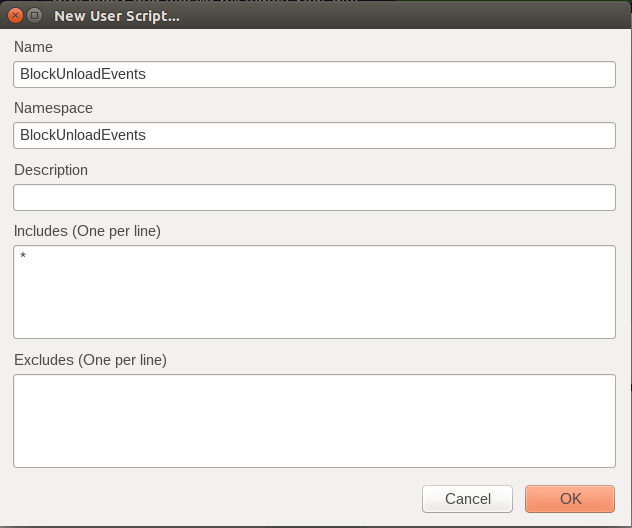
\includegraphics[width=0.5\textwidth]{pictures/greasymonkey-script.png}
  \caption{Creating a new user script with Greasymonkey}
  \label{fig:greasymonkey_script}
\end{figure}

\newpage
\begin{listing}
\begin{verbatim}
// ==UserScript==
// @name        BlockUnloadEvents
// @namespace   BlockUnloadEvents
// @include     *
// @version     1
// @grant       none
// ==/UserScript==
(function() {
  unsafeWindow.onbeforeunload = null;
  unsafeWindow.onunload = null;
})();
\end{verbatim}
\caption{BlockUnloadEvents.js}
\end{listing}

\begin{listing}
\begin{verbatim}
// ==UserScript==
// @name        OverwriteAlert
// @namespace   OverwriteAlert
// @include     *
// @version     1
// @grant       none
// @run-at      document-start
// ==/UserScript==
unsafeWindow.alert = function(){};
unsafeWindow.confirm = function(){};
unsafeWindow.prompt = function(){};
\end{verbatim}
\caption{OverwriteAlert.js}
\end{listing}
